\chapter{Detectors\label{chap:det}}

\section{Overview}

The beamline software is compatible with Amptek detector assemblies which use
the DP5 Pulse Processor and MCA board\cite{dp5_user_man}, including the
XR-100\cite{xr-100-sdd-manual} and the
X-123\cite{x-123-sdd-manual,x-123-cdte-manual} models, both of which come in
silicon drift (SDD) or cadmium telluride (CdTe) detector varieties. The XR-100
and X-123 models are very similar, except the digital pulse processor and power
supply in the XR-100 are separate from the detector and preamplifier, while in
the X-123, everything is integrated into a single package.

The SDD and CdTe detector are useful for different situations and energy ranges
of interest. The SDD has overall better resolution and lower noise, and is more
efficient than the CdTe detector at low energies. The CdTe detector has a lower
resolution and is more prone to noise at lower energies, but it is much more
efficient at high energies. As a rule of thumb, the SDD should be used for
measuring energies below about 25~keV, and the CdTe for energies higher than
25~keV.

Any of the detector models from Amptek listed above can be mounted onto the
detector stage assembly, powered up as specified in the manual, and connected to
the computer via RS-232. The \texttt{blcontrol} software should automatically
connect to the detector when next powered up; if not, try modifying the
\texttt{serialport} configuration variable in \texttt{config/blconf.txt}.

The detectors are rather fragile and it is important to handle them with
care. In particular, they are very sensitive to any sort of mechanical shock, so
it is important to not drop them during mounting, or allow them to run into any
other elements of the beamline during alignment. The beryllium window on the end
of the detector housing is also easily damaged. It is recommended to keep the
red protective cap or a tungsten cap with no pinhole on the end of the detector
when it is not in use. The detector diode is held under vacuum behind the Be
window and cooled by a thermoelectric cooler (TEC). The detector has best performance
(best resolution and least noise) when kept at a temperature below 225K. If the
set point is below 225K but the TEC is unable to cool the detector to this
temperature, this could indicate damage to the TEC or loss of vacuum, and the
detector will likely need to be serviced by the manufacturer.

\section{Calibration\label{sec:calib}}

Each detector needs to be calibrated every few weeks or after a long period of
disuse. To calibrate the detector, we measure sealed sources with known spectral
lines and correlate the MCA channels of these lines with their energies.

\subsection{Collecting calibration spectra}

Any source with spectral lines in the energy range of interest can be
used for calibration. At the time of this writing, we are calibrating
all detectors with three sealed sources: $^{55}$Fe, which has spectral
lines at 5.9 and 6.5 keV; $^{57}$Co, with a line at 14.4 keV; and
$^{137}$Cs, which has a line at 32.2 keV.

For calibration, a long spectrum (at least 10 minutes) will be
acquired with every source following the steps below.
\begin{enumerate}
\item Start up the software and adjust the detector gain so that all
  peaks from the sources you are using will be within the detector's
  energy range.
\item \label{itm:affix} Using tape, affix one of the sources to the
  mylar on the end of the Cu pipe near the detector. Using the knobs
  on the stages, move the detector so that the Be window is close to
  the source.
\item In the software, acquire a short spectrum (30 seconds to 1 minute) to
  ensure that the source peaks are visible and the detector dead time is not too
  high (should be <5\%). You should use a large number of channels to get the
  best possible resolution---8192 is best. If necessary, move the detector and
  take another short spectrum.
\item \label{itm:acquire} Acquire a long spectrum with the same number of
  channels for at least 10 minutes, and then save it.
\item \label{itm:reacquire} If the peaks in this 10 minute spectrum
  are still not very well resolved, take another spectrum for 10
  minutes or more. All spectra from a given sample can be added
  together for better statistics during the analysis.
\item After saving the spectrum from the previous source, remove the
  source and repeat steps \ref{itm:affix}-\ref{itm:reacquire} with a new
  source. Make sure to use the same gain and the same number of
  channels for each source. The acquisition time can vary from source
  to source. Repeat with all sealed sources.
\item When finished with the sealed sources, put them away in the lead
  source holder and place the holder in a locked cabinet.
\end{enumerate}
  
\subsection{Calibration data analysis}

%outline calib script
The script \path{blcontrol/scripts/calib.py} assists with the detector
calibration by fitting the peaks in each source spectrum, and then
fitting each of these peaks to a line which defines the detector
calibration parameters. The energy as a funciton of channel number,
$E(C)$, is found by fitting the source peak channels to a function of
the form
\begin{equation}
  \label{eq:calib-lin}
  E(C) = \frac{ C }{ \alpha \times G \times N } + E_0 \,
\end{equation}
where $G$ is the hardware gain and $N$ is the total number of channels. $\alpha$
and $E_0$, called the calibration factor and the offset, respectively, are
fitting parameters. Figures~\ref{fig:co57} and \ref{fig:linfit} show examples of
the plots output by the calibration script. The script will also print the
calculated values of the calibration factor and offset. You should inspect the
outputs to ensure that the values printed are sensible. Then,to enable the
calibration, paste these values into the appropriate location in
\texttt{blconf.txt} for the detector that you are calibrating. 

\begin{figure}
  \centering
  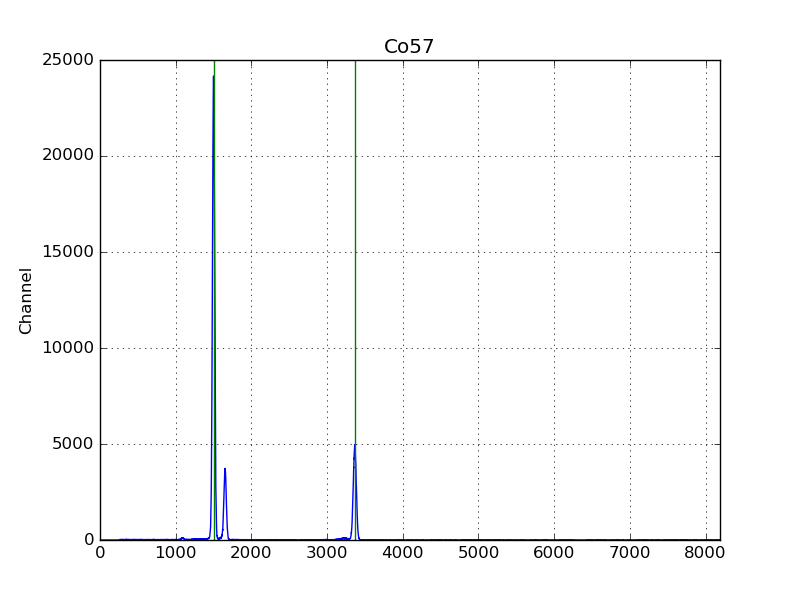
\includegraphics[width=0.7\textwidth]{Co57.png}
  \caption{\label{fig:co57} An example of a calibration spectrum from $^{57}$Co,
    with the peaks highlighted.}
\end{figure}

\begin{figure}
  \centering
  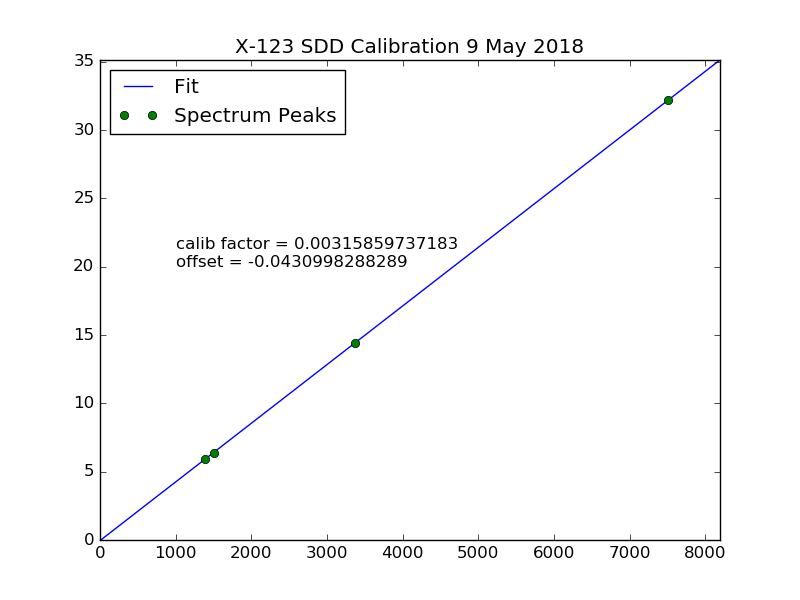
\includegraphics[width=0.7\textwidth]{linfit.png}
  \caption{\label{fig:linfit} This plot shows a linear fit to the peak channel
    as a function of energy for multiple calibration sources, calculated by the
    script \texttt{calib.py}. }
\end{figure}


%show example output plot

%%% Local Variables:
%%% mode: latex
%%% TeX-master: "Beamline_Manual"
%%% End:
